\documentclass[a4paper, 12pt]{article}

% <--------- Packages ---------> %

\usepackage{fullpage}   % Package to use full page
\usepackage{tikz}       % Package for drawing
\usepackage{pdfpages}
\usepackage{fancyhdr}
\usepackage{array}
\usepackage{tabularx}
\usepackage{colortbl}
\usepackage{pgfplots}
\usepackage{xcolor}
\usepackage{float}

% <--------- Mathematics ---------> %

\usepackage{amssymb}   % Extra symbols
\usepackage{amsthm}  
\usepackage{amsmath}   % Theorem-like environments
\usepackage{thmtools}  % Theorem-like environments
\usepackage{mathtools} % Fonts and environments for mathematical formuale
\usepackage{mathrsfs}  % Script font with \mathscr{}

% <--------- Others ---------> %

\usepackage{indentfirst}
\usepackage[utf8]{inputenc}
\usepackage[english]{babel}
\usepackage[thinlines]{easytable}
\usepackage{caption}
% \usepackage[parfill]{parskip}
\usepackage{pgfplots}


%===========================================%
%=            Page Style                   =%

\usepackage{times}

\pgfplotsset{compat=1.7}
\setlength{\parindent}{1.3em}
\renewcommand{\baselinestretch}{1.5}

%=                                         =%
%===========================================%


%===========================================%
%=            Code Setup                   =%

\usepackage{listings}
\usepackage{color}

\definecolor{dkgreen}{RGB}{163, 190, 140}
\definecolor{gray}{RGB}{59, 66, 82}
\definecolor{mauve}{RGB}{94, 129, 172}
\definecolor{lightgray}{RGB}{46, 52, 64}

\lstset{
  language={Python},
  aboveskip=0.6mm,
  belowskip=0.6mm,
  showstringspaces=false,
  columns=flexible,
  basicstyle={\small\ttfamily},
  numbers=left,
  numberstyle=\tiny\color{gray},
  keywordstyle=\color{mauve},
  commentstyle=\color{gray},
  stringstyle=\color{dkgreen},
  morekeywords={pop},
  breaklines=true,
  breakatwhitespace=true,
  tabsize=4
}

%=                                         =%
%===========================================%


%===========================================%
%=               Credits                   =%

\author{Name}
\title{Title}

%=                                         =%
%===========================================%

%===========================================%
%=               BEGIN                     =%

\begin{document}

\pgfplotsset{compat=1.17}
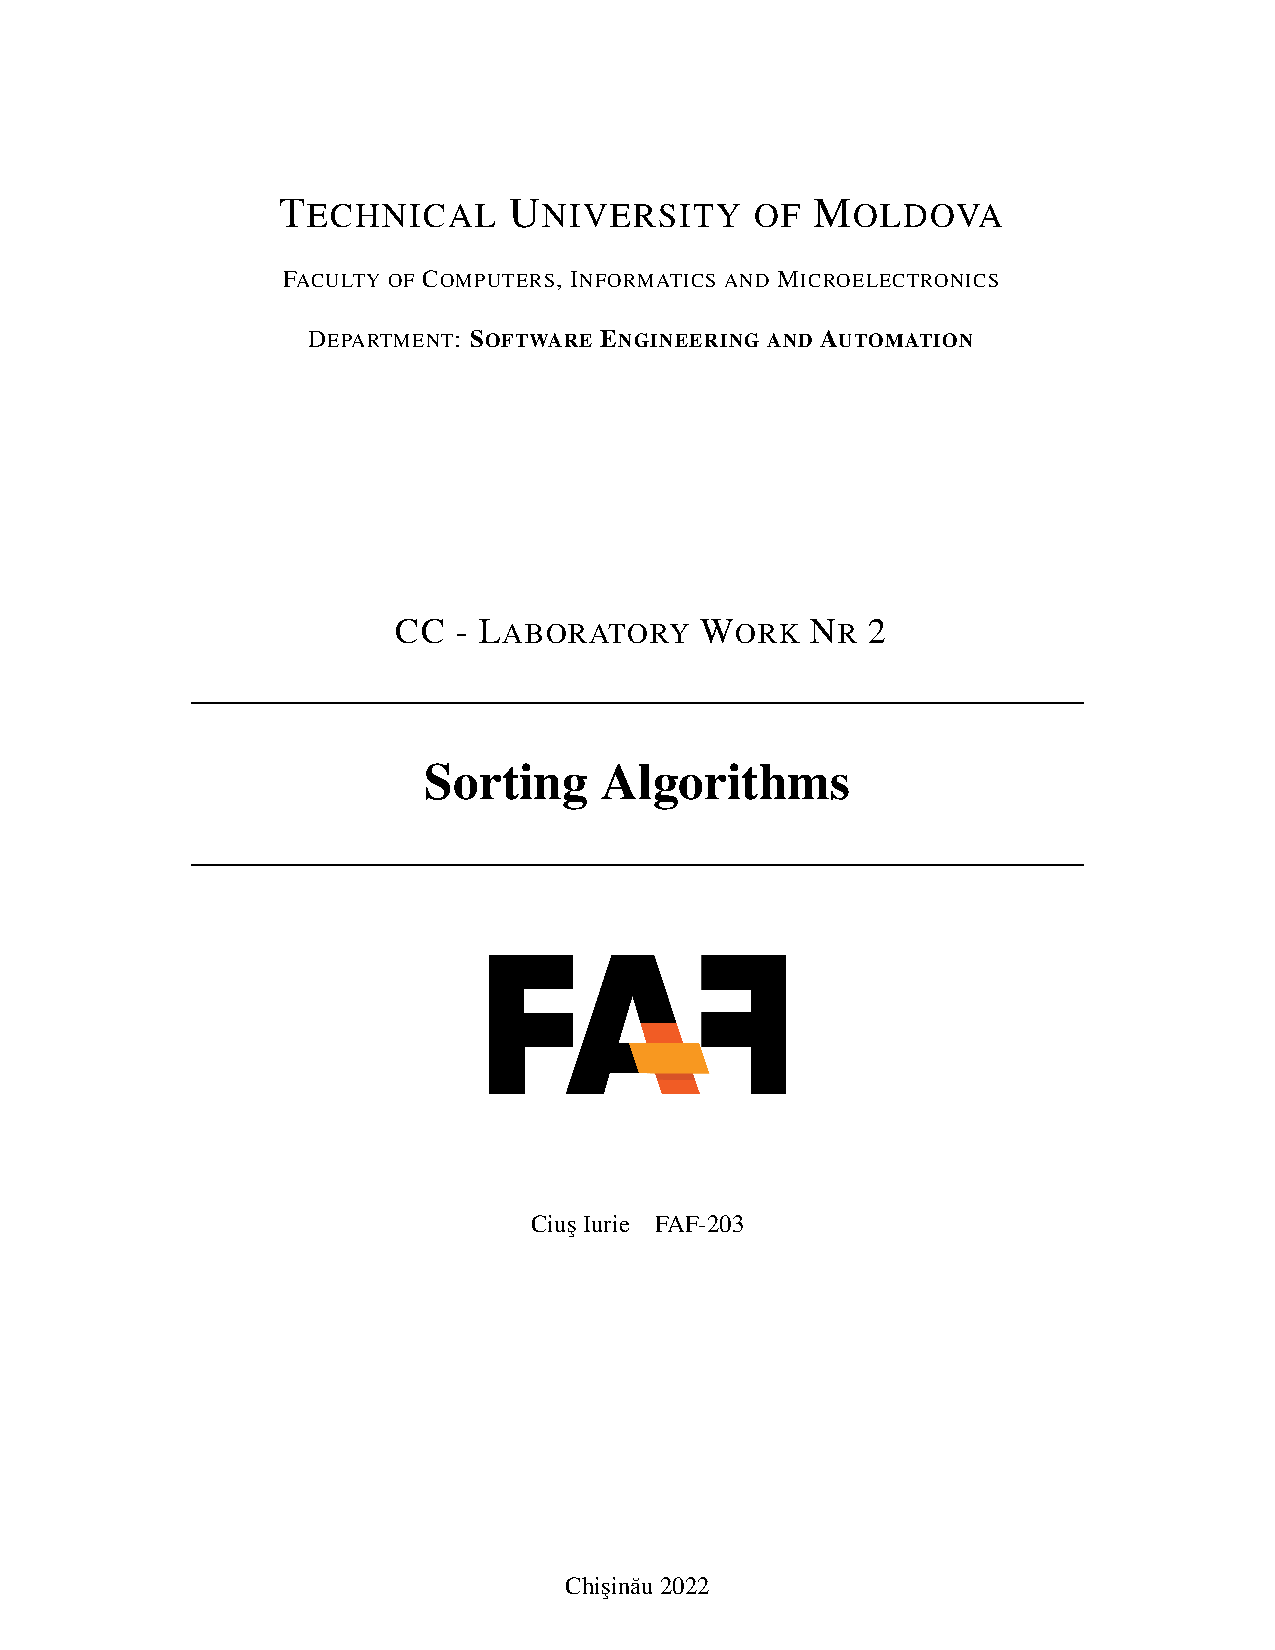
\includepdf[pages={1}]{title.pdf}
\tableofcontents

\newpage

\section{Algorithm Analysis}

Algorithm analysis is an important part of computational complexity theory, which provides
theoretical estimation for the required resources of an algorithm to solve a specific computational problem. Analysis of algorithms is the determination of the amount of time and space
resources required to execute it.

\subsection{Introduction}

The current paper work represents my implementation of four sorting algorithms. 

\hfill \break
\indent A Sorting Algorithm is used to rearrange a given array or list elements according to a comparison operator on the elements. The comparison operator is used to decide the new order of element in the respective data structure.

From the beginning of computing, the sorting problem has attracted 
a great deal of research, perhaps due to the complexity of solving 
it efficiently despite its simple, familiar statement. Among the 
authors of early sorting algorithms around 1951 was Betty Holberton, 
who worked on \textbf{ENIAC} and \textbf{UNIVAC}. Bubble sort was analyzed as early 
as 1956. Asymptotically optimal algorithms have been known since the 
mid-20th century - new algorithms are still being invented, with the 
widely used Timsort dating to 2002, and the library sort being first 
published in 2006.

Comparison sorting algorithms have a fundamental requirement of $\Omega(nlogn)$
comparisons (some input sequences will require a multiple of n log n comparisons, 
where n is the number of elements in the array to be sorted). Algorithms not based 
on comparisons, such as counting sort, can have better performance.

Sorting algorithms are prevalent in introductory computer science classes, 
where the abundance of algorithms for the problem provides a gentle introduction 
to a variety of core algorithm concepts, such as big O notation, divide and conquer 
algorithms, data structures such as heaps and binary trees, randomized algorithms, 
best, worst and average case analysis, time-space tradeoffs, and upper and lower bounds.

Sorting small arrays optimally (in fewest comparisons and swaps) or fast 
(i.e. taking into account machine specific details) is still an open research 
problem, with solutions only known for very small arrays (<20 elements). 
Similarly optimal (by various definitions) sorting on a parallel machine is 
an open research topic.

\subsection{Objectives}

\begin{itemize}
  \item Study and empirical analysis of sorting algorithms. QuickSort, mergeSort, heapSort analysis, (one of your choice).
  \item Establish the properties of the input data in relation to which the analysis is made.
  \item Choose the metric for comparing algorithms.
  \item Perform empirical analysis of the proposed algorithms.
  \item Make a conclusion on the work done.
\end{itemize}

\subsection{Theoretical Notes}

An algorithm is correct if for any instance of it
ends with a correct output which is the solution to the calculation problem
solved by the respective algorithm. Some algorithms, however, are incorrect
In the sense that they do not lead to any finite time solution or lead to
Wrong solutions, they can be useful as long as the errors they produce can be
controlled.

The behavior of the same algorithm may be different depending on
input data. That is why great attention must be paid to them
the latter. A variable present in the input of an algorithm can
identify an array or object of a composite data and it will be treated
as a pointer to the elements of the painting, respectively to the fields
(attributes) of the corresponding object.

How to define the size of the input data
depends on the calculated calculation problem. It can be expressed by:

\begin{itemize}
  \item the number of items contained in the input data (for example,
  the size of an array of integers);
  \item the total number of bits in the binary representation of the data
  entry;
  \item two natural numbers
\end{itemize}

For each algorithm that solves a certain problem P
it is necessary to specify how the input data size is expressed.

If there is an algorithm that solves the problem P it doesn't mean he is unique.

For example, there are algorithms like: \textbf{QuickSort}, \textbf{MergeSort}, \textbf{TreeSort},
sorting by selection and insertion etc. which are used for the same purpose.

Therefore, there is a need to choose an algorithm from
the class of algorithms that solve the problem P corresponding to some
requirements. The algorithm depends on the application, implementation, environment,
frequency of use etc. Comparing algorithms is a process
subtle that has several aspects in mind. Next, we'll look at some ways to implement 
a few of the most popular sorting algorithms.

\newpage

\subsection{Algorithms}

\subsubsection{QuickSort}

QuickSort is a Divide and Conquer algorithm. It picks an element as pivot 
and partitions the given array around the picked pivot. There are many different 
versions of quickSort that pick pivot in different ways. 

\begin{enumerate}
  \item Always pick first element as pivot.
  \item Always pick last element as pivot.
  \item Pick a random element as pivot.
  \item Pick median as pivot (implemented below).
\end{enumerate}

\begin{lstlisting}
  /* low  --> Starting index,  high  --> Ending index */
  quickSort(arr[], low, high)
  {
      if (low < high)
      {
          /* pi is partitioning index, arr[pi] is now
            at right place */
          pi = partition(arr, low, high);

          quickSort(arr, low, pi - 1);  // Before pi
          quickSort(arr, pi + 1, high); // After pi
      }
  }
\end{lstlisting}

\newpage

\subsubsection{Merge Sort}

Like QuickSort, Merge Sort is a Divide and Conquer 
algorithm. It divides the input array into two halves, 
calls itself for the two halves, and then merges the two sorted halves. 
The merge() function is used for merging two halves. The merge(arr, l, m, r) 
is a key process that assumes that arr[l..m] and arr[m+1..r] are sorted and 
merges the two sorted sub-arrays into one.

\begin{lstlisting}
  MergeSort(arr[], l,  r)
  If r > l
      1. Find the middle point to divide the array into two halves:  
              middle m = l+ (r-l)/2
      2. Call mergeSort for first half:   
              Call mergeSort(arr, l, m)
      3. Call mergeSort for second half:
              Call mergeSort(arr, m+1, r)
      4. Merge the two halves sorted in step 2 and 3:
              Call merge(arr, l, m, r)
\end{lstlisting}

The following diagram from wikipedia shows the complete merge sort process 
for an example array {38, 27, 43, 3, 9, 82, 10}. If we take a closer look 
at the diagram, we can see that the array is recursively divided into two 
halves till the size becomes 1. Once the size becomes 1, the merge processes 
come into action and start merging arrays back till the complete array is merged.

\begin{center}
  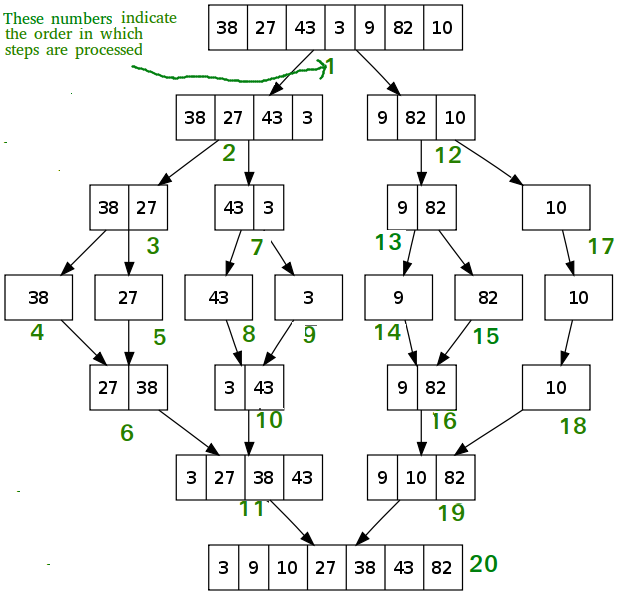
\includegraphics[width=7cm]{merge.png}
\end{center}

\newpage

\subsubsection{Heap Sort}

Heap sort is a comparison-based sorting technique based on 
Binary Heap data structure. It is similar to selection sort 
where we first find the minimum element and place the minimum element 
at the beginning. We repeat the same process for the remaining elements.

\subparagraph{What is Binary Heap?}

\hfill \break
\indent A \textbf{binary heap} is a heap, i.e, a tree which obeys 
the property that the root of any tree is greater 
than or equal to (or smaller than or equal to) all 
its children (heap property). The primary use of such a data structure is 
to implement a priority queue.

\subparagraph{How to “heapify” a tree?}

\hfill \break
\indent The process of reshaping a binary tree into a Heap data structure is known 
as \textbf{heapify}. A binary tree is a tree data structure that has two child nodes at max. 
If a node's children nodes are \textbf{heapified}, then only \textbf{heapify} process can be applied 
over that node. A heap should always be a complete binary tree. 

Starting from a complete binary tree, we can modify it to become a Max-Heap by 
running a function called \textbf{heapify} on all the non-leaf elements of the heap. i.e. 
\textbf{heapify} uses recursion.

\hfill \break
\begin{lstlisting}
   heapify(array)
   Root = array[0]
   Largest = largest( array[0] , array [2 * 0 + 1]. array[2 * 0 + 2])
   if(Root != Largest)
       Swap(Root, Largest)
\end{lstlisting}

\newpage

\subsubsection{Cocktail Sort}

Cocktail Sort is a variation of Bubble sort. 
Bubble sort algorithm always traverses elements from left 
and moves the largest element to its correct position in first 
iteration and second largest in second iteration and so on. Cocktail 
Sort traverses through a given array in both directions alternatively. 

Each iteration of the algorithm is broken up into 2 stages: 

\begin{enumerate}
  \item The first stage loops through the array from left to right, just like the Bubble Sort. During the loop, adjacent items are compared and if value on the left is greater than the value on the right, then values are swapped. At the end of first iteration, largest number will reside at the end of the array.
  \item The second stage loops through the array in opposite direction- starting from the item just before the most recently sorted item, and moving back to the start of the array. Here also, adjacent items are compared and are swapped if required.
\end{enumerate}

\newpage

\section{Code}

\subsection{Implementation}

\lstinputlisting[language=Python]{../SORTLIB.py}

\subsection{Time Complexity}

\subsubsection*{Quick Sort}
\begin{itemize}
  \item \textbf{Worst Case}: The worst case occurs when the partition process always picks greatest or smallest element as pivot. If we consider above partition strategy where last element is always picked as pivot, the worst case would occur when the array is already sorted in increasing or decreasing order. \textbf{\textit{$\Omega(n^2)$}}. 
  \item \textbf{Best Case}: The best case occurs when the partition process always picks the middle element as pivot. Following is recurrence for best case: $O(n\cdot log(n))$
\end{itemize}

\subsubsection*{Merge Sort}

Time Complexity: Sorting arrays on different machines. Merge Sort is a recursive algorithm and time complexity can be expressed as following recurrence relation. 

$$
  T(n) = 2T\frac{n}{2} + O(n)
$$

The above recurrence can be solved either using the Recurrence Tree method or the Master method. It falls in case II of Master Method and the solution of the recurrence is $O(n\cdot log(n))$. Time complexity of Merge Sort is  $O(n\cdot log(n))$ in all 3 cases (worst, average and best) as merge sort always divides the array into two halves and takes linear time to merge two halves.

\subsubsection*{Heap Sort}

Time complexity of heapify is $O(log(n))$. Time complexity of createAndBuildHeap() is O(n) and the overall time complexity of Heap Sort is $O(n\cdot log(n))$.

\subsubsection*{Cocktail Sort}

\begin{itemize}
  \item \textbf{Worst and Average Case Time Complexity:} $O(n^2)$. 
  \item \textbf{Best Case Time Complexity:} $O(n)$. Best case occurs when array is already sorted.
\end{itemize}

\newpage

\subsection{Graphs}

\begin{center}
  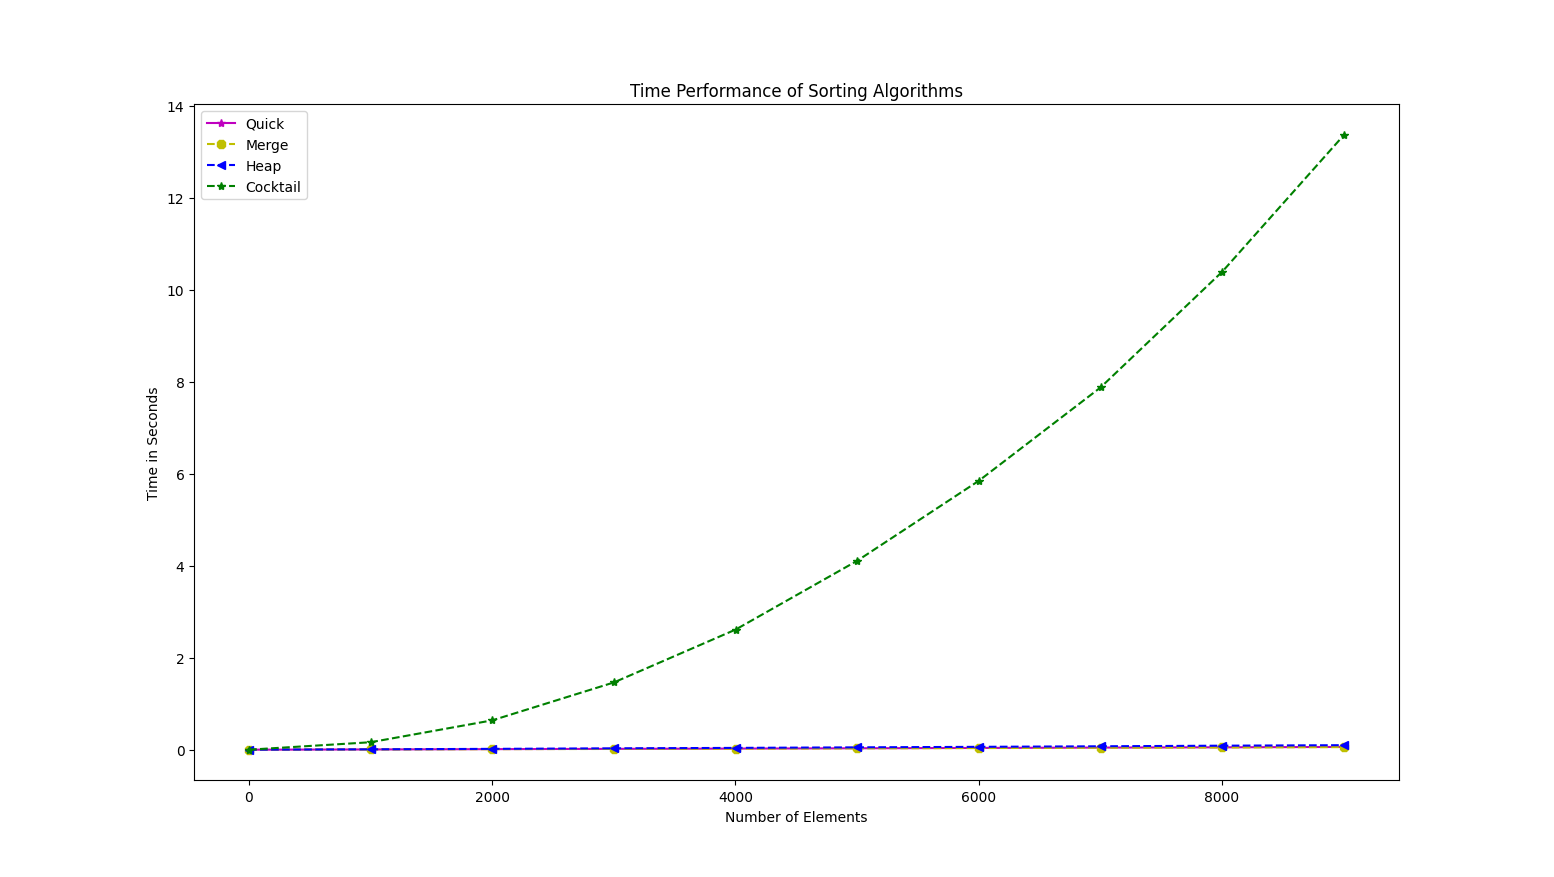
\includegraphics[width=15cm]{graph.png}
\end{center}

\section{Conclusion}

During this laboratory work, I studied and analyzed four 
of the most popular sorting algorithms, each with it's upsides and downsides. 
Efficient sorting is important for optimizing the efficiency of other 
algorithms (such as search and merge algorithms) 
that require input data to be in sorted lists. Sorting is also often 
useful for canonicalizing data and for producing human-readable output.

I have tested all the algorithm on 10 arrays within a range of 0 to 10000 elements, 
randomly generated from 0 to 200. Based on the results and the computing time, I can 
say that the \textbf{Cocktail Sort} performed the worst with a time complexity of \textit{nlogn}. 
Meanwhile the rest of them performed too good, almost close to 0. Which is why I am unable 
to tell which is the fastest. But in my opinion, the \textbf{Merge Sort} was easier to implement.

\subsection{References}

\begin{itemize}
  \item https://github.com/IuraCPersonal/FAF203-CC
\end{itemize}


\end{document}

%=                END                      =%
%===========================================%